\subsection{Resultados de la simulaciones}
\subsubsection{Materiales sin defectos}
\frame{
	\frametitle{Materiales sin defectos}
	\framesubtitle{PtSe\textsubscript{2} y PtS\textsubscript{2}}
	\begin{table}[!hbt]
		\centering
		\begin{tabular}{|c||c|c|c|}
			\hline
			Material & Celda & Constante de Red (\AA) &Magnetizaci\'on\\
			\hline
			\hline
			PtSe\textsubscript{2} & 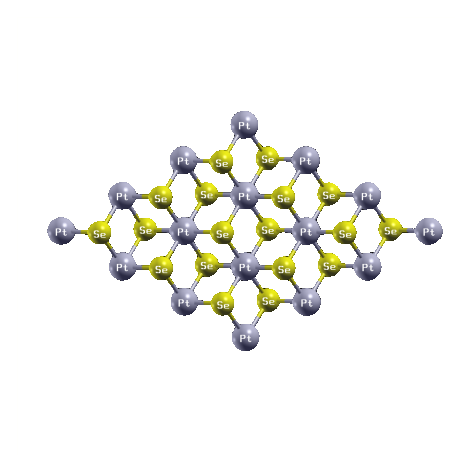
\epsfig{file=figRes/PtSe2/est/est1.eps, scale=0.3}& $3.7610$&$0\mu_{B}/celda$ \\
			\hline
			PtS\textsubscript{2} & 	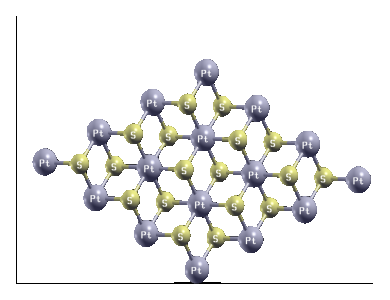
\epsfig{file=figRes/PtS2/parCelU.eps, scale=0.3}& $3.5785$&$0\mu_{B}/celda$\\
			\hline
		\end{tabular}
	\end{table}
}

\frame{
	\frametitle{Materiales sin defectos}
	\framesubtitle{VSe\textsubscript{2} y VS\textsubscript{2}}
	\begin{table}[!hbt]
		\centering
		\begin{tabular}{|c||c|c|c|}
			\hline
			Material & Celda &Constante de Red (\AA)& Magnetizaci\'on \\
			\hline
			\hline
			VSe\textsubscript{2} & 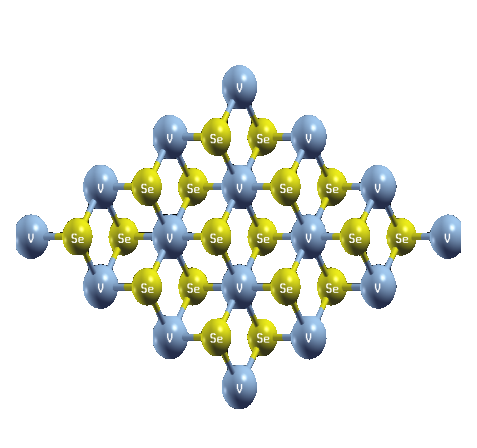
\epsfig{file=figRes/VSe2/par.png.eps, scale=0.3}&$3.3403$ & $0.62\mu_{B}/celda$\\
			\hline
			VS\textsubscript{2} & 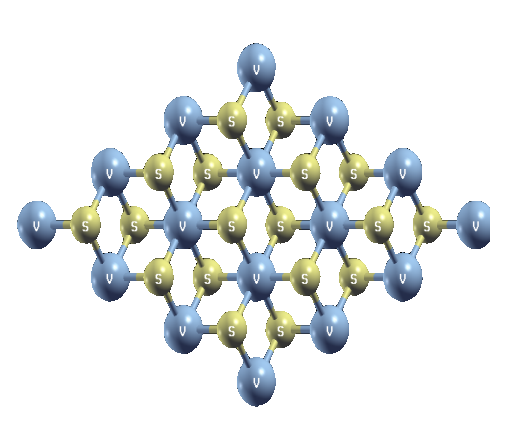
\epsfig{file=figRes/VS2/par.eps, scale=0.3}&$3.1939$ &$0.55\mu_{B}/celda$\\
			\hline
		\end{tabular}
	\end{table}
}
\frame{
	\frametitle{VSe\textsubscript{2}}
	\framesubtitle{Diagrama de Bandas y Densidad de estados}
	\begin{figure}
		\includegraphics[scale=0.6]{figRes/VSe2/bandas/celU/nosoc/bandasDOSnoSoc.pdf}
		\label{Sim:fig:bandnoSocVse2}
		\caption{Diagrama de bandas y densidad de estados del VSe\textsubscript{2} sin efecto spin-\'orbita.}
	\end{figure}	
}
\frame{
	\frametitle{VS\textsubscript{2}}
	\framesubtitle{Diagrama de Bandas y Densidad de estados}
	\begin{figure}
		\includegraphics[scale=0.6]{figRes/VS2/celdaU/estructura electronica/noSOC/bandasDOSnoSoc.pdf}
		\label{Sim:fig:bandnoSocVs2}
		\caption{Diagrama de bandas y densidad de estados del VS\textsubscript{2} sin efecto spin-\'orbita.}
	\end{figure}	
}
\frame{
	\frametitle{VSe\textsubscript{2}}
	\framesubtitle{Densidad de spin}
	\begin{figure}[!hbt]
		\centering
		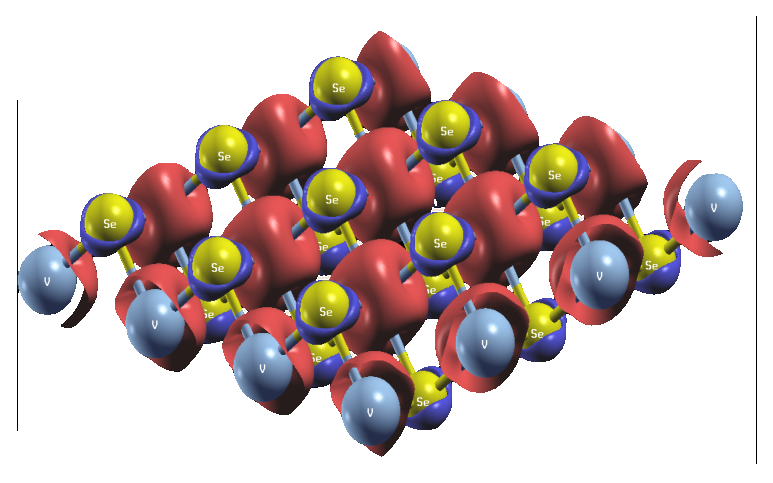
\epsfig{file=figRes/VSe2/vse2magz.eps, scale=0.5}
		\caption[Distribuci\'on de spin en VSe\textsubscript{2}]{Distribuci\'on  de spin en el VSe\textsubscript{2}.}
		\label{Sim:fig:distmagnVse2}
	\end{figure}
}
\frame{
	\frametitle{VS\textsubscript{2}}
	\framesubtitle{Densidad de spin}
	\begin{figure}[!hbt]
		\centering
		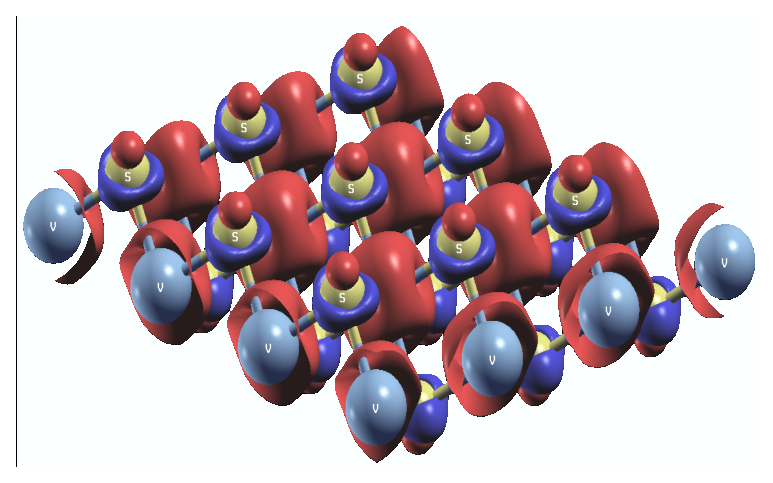
\epsfig{file=figRes/VS2/vs2magz.eps, scale=0.5}
		\caption[Densidad de spin en el VS\textsubscript{2}.]{Distribuci\'on  de spin en el VS\textsubscript{2}.}
		\label{Sim:fig:distmagnVs2}
	\end{figure}
}
\subsubsection{Estudio de vacancia de metal de transici\'on}
\frame{
    \frametitle{Vacancia de Platino en PtSe\textsubscript{2} y PtS\textsubscript{2}}
	\begin{table}[!hbt]
		\centering
		\begin{tabular}{|c||c|c|}
			\hline
			Material & Celda & Momento magn\'etico \\
			\hline
			\hline
			PtSe\textsubscript{2} &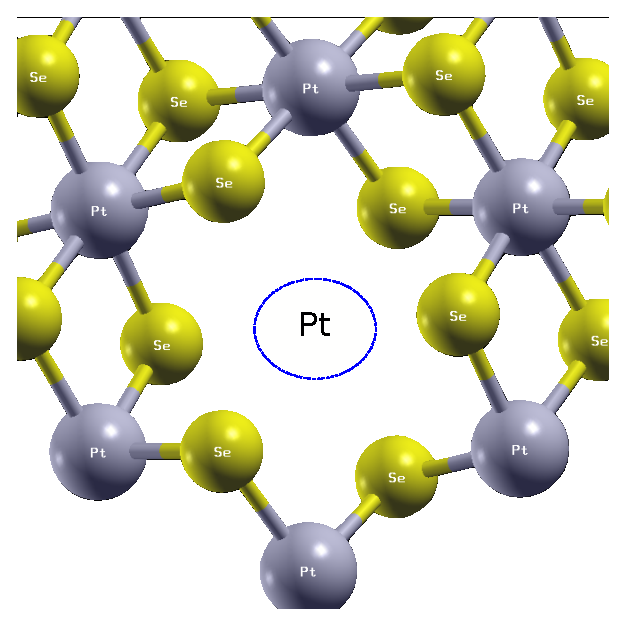
\epsfig{file=figRes/PtSe2/VacanciaPt.eps, scale=0.3}& $2.37\mu_{B}/celda$\\
			\hline
			PtS\textsubscript{2} &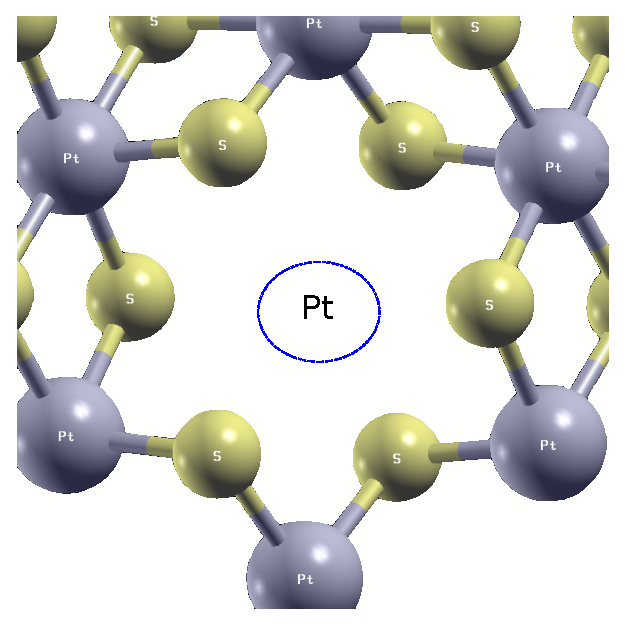
\epsfig{file=figRes/PtS2/VacanciaPt.eps, scale=0.3}& $2.63\mu_{B}/celda$\\
			\hline
		\end{tabular}
	\end{table}
}
\frame{
	\frametitle{Vacancia de Platino en PtSe\textsubscript{2} y PtS\textsubscript{2}}
	\framesubtitle{Densidad de carga}
	
	\begin{figure}[!hbt]
		\centering
		\subfigure[PtSe\textsubscript{2}]{
			\includegraphics[scale=0.45]{figRes/PtSe2/densidades/densPos/densidadpos.pdf}
			\label{Sim:fig:cargavacPtse2}
		}
		\subfigure[PtS\textsubscript{2}]{
			\includegraphics[scale=0.45]{figRes/PtS2/def/densidades/denspos/densidadpos.pdf}
			\label{Sim:fig:cargavacPts2}
		}
		\caption[Distribuci\'on de carga en alrededor de la vacancia de platino en PtSe\textsubscript{2} y PtSe\textsubscript{2}.]{Distribuci\'on de carga alrededor de la vacancia de platino en PtSe\textsubscript{2} (\ref{Sim:fig:cargavacPtse2}), y en PtS\textsubscript{2} (\ref{Sim:fig:cargavacPtse2}).}
		\label{Sim:fig:cargavac}	
	\end{figure}
}

\frame{
	\frametitle{Vacancia de Platino en PtSe\textsubscript{2} y PtS\textsubscript{2}}
	\framesubtitle{Diagrama de bandas y densidad de estados del PtSe\textsubscript{2}}
	
	\begin{figure}[!hbt]
		\centering
		\includegraphics[scale=0.7]{figRes/PtSe2/def/bandas/nosoc/bandasDOSnoSoc.pdf}
		\caption[Diagrama de bandas y densidad de estados del PtSe\textsubscript{2} con vacancia de Platino.]{Diagrama de bandas y densidad de estados sin incluir el efecto de spin \'orbita en el PtSe\textsubscript{2}.}
		\label{Sim:fig:bandDefPtse2noSOC}
	\end{figure}
}
\frame{
	\frametitle{Vacancia de Platino en PtSe\textsubscript{2} y PtS\textsubscript{2}}
	\framesubtitle{Diagrama de bandas y densidad de estados del PtS\textsubscript{2}}
	\begin{figure}[!hbt]
		\centering
		\includegraphics[scale=0.7]{figRes/PtS2/def/bandas/nosoc/bandasDOSnoSoc.pdf}
		\caption[Diagrama de bandas y densidad de estados del PtS\textsubscript{2} con una vacancia de Platino.]{Diagrama de bandas y densidad de estados del PtS\textsubscript{2}.  }
		\label{Sim:fig:noSOCpts2def}
	\end{figure}
}
\frame{
	\frametitle{Vacancia de Platino en PtSe\textsubscript{2} y PtS\textsubscript{2}}
	\framesubtitle{Densidad de carga y de spin en PtSe\textsubscript{2}}
	\begin{figure}[!hbt]
		\centering
		\subfigure[densidad de carga]{
			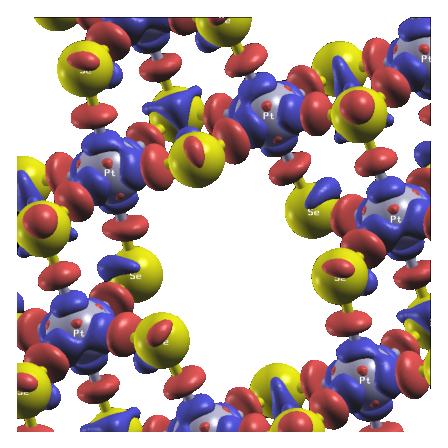
\epsfig{file=figRes/PtSe2/def/ptse2_carga, scale=0.6}
			\label{Sim:fig:CargaVacPtse2}
		}
		\subfigure[densidad de spines]{
			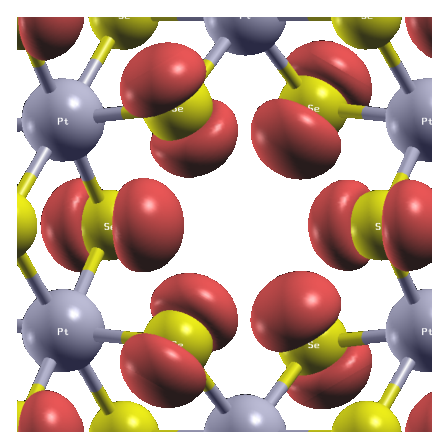
\epsfig{file=figRes/PtSe2/def/ptse2_magz, scale=0.6}
			\label{Sim:fig:MagzVacPtse2}
		}
		\caption[Iso superficies de la densidad de carga y de spin en el PtSe\textsubscript{2} con vacancia de Platino.]{Isosuperficies de la densidad de carga (\ref{Sim:fig:CargaVacPtse2}) y la densidad de spines (\ref{Sim:fig:MagzVacPtse2} del PtSe\textsubscript{2} con un valor de $0.001 e/\AA^3$. }
	\end{figure}
}

\frame{
	\frametitle{Vacancia de Platino en PtSe\textsubscript{2} y PtS\textsubscript{2}}
	\framesubtitle{Densidad de carga y de spin en PtS\textsubscript{2}}
	\begin{figure}[!hbt]
		\centering
		\subfigure[densidad de carga]{
			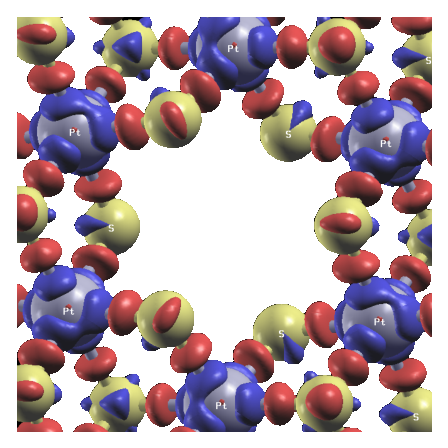
\epsfig{file=figRes/PtS2/def/densidades/pts2_carga, scale=0.6}
			\label{Sim:fig:CargaVacPts2}
		}
		\subfigure[densidad de spines]{
			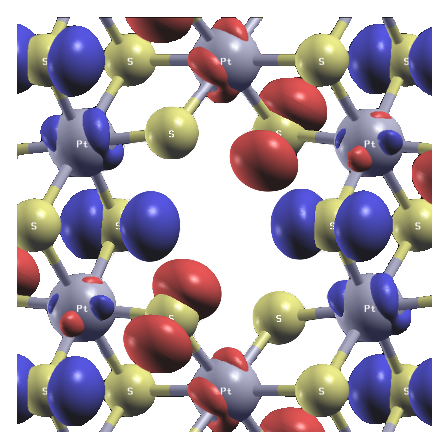
\epsfig{file=figRes/PtS2/def/densidades/pts2_magz, scale=0.6}
			\label{Sim:fig:MagzVacPts2}
		}
		\caption[Iso superficies de la densidad de carga y de spin en el PtS\textsubscript{2} con vacancia de Platino.]{Isosuperficies de la densidad de carga (\ref{Sim:fig:CargaVacPts2}) y la densidad de spines (\ref{Sim:fig:MagzVacPts2} del PtS\textsubscript{2} con un valor de $0.001 e/\AA^3$. }
	\end{figure} 
}
\frame{
	\frametitle{Vacancia de Vanadio en VSe\textsubscript{2} y VS\textsubscript{2}}
	\begin{table}[!hbt]
		\centering
		\begin{tabular}{|c||c|c|}
			\hline
			Material & Celda & Momento magn\'etico \\
			\hline
			\hline
			VSe\textsubscript{2} & 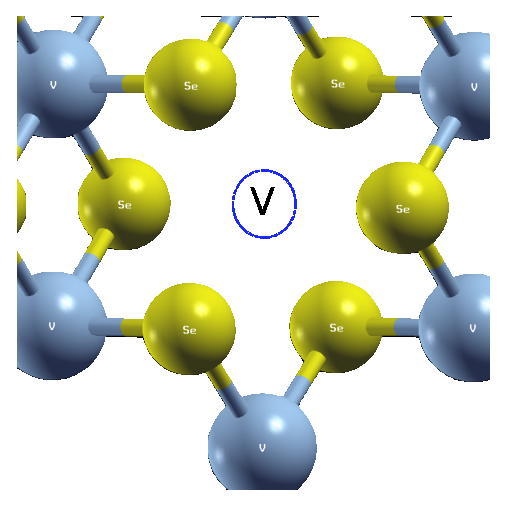
\epsfig{file=figRes/VSe2/def/vacVse2_def, scale=0.34}& $0.48\mu_{B}/celda$\\
			\hline
			VS\textsubscript{2} & 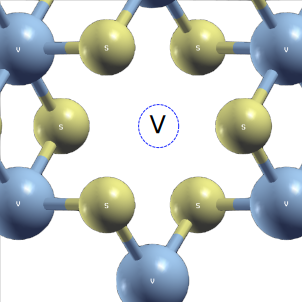
\epsfig{file=figRes/VS2/def/vs2_def, scale=0.34}& $0.76\mu_{B}/celda$\\
			\hline
		\end{tabular}
	\end{table}
}

\frame{
	\frametitle{Vacancia de Vanadio en VSe\textsubscript{2} y VS\textsubscript{2}}
	\framesubtitle{Densidad de carga}
	
	\begin{figure}[!hbt]
		\centering
		\subfigure[VSe\textsubscript{2}]{
			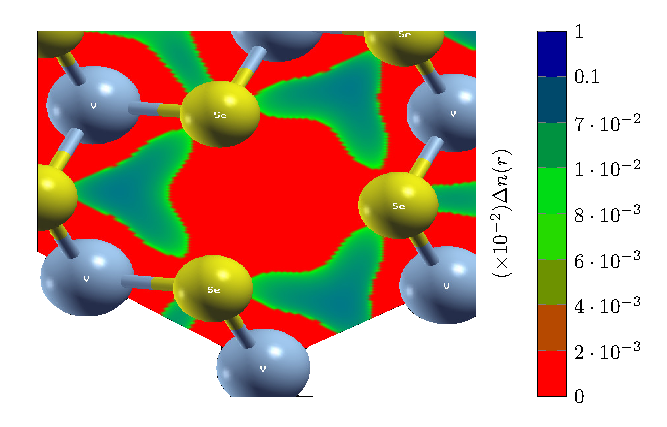
\epsfig{file=figRes/VSe2/def/densidad/densPos/densidadpos, scale=0.45}
			\label{Sim:fig:cargavacVSe2}
		}
		\subfigure[VS\textsubscript{2}]{
			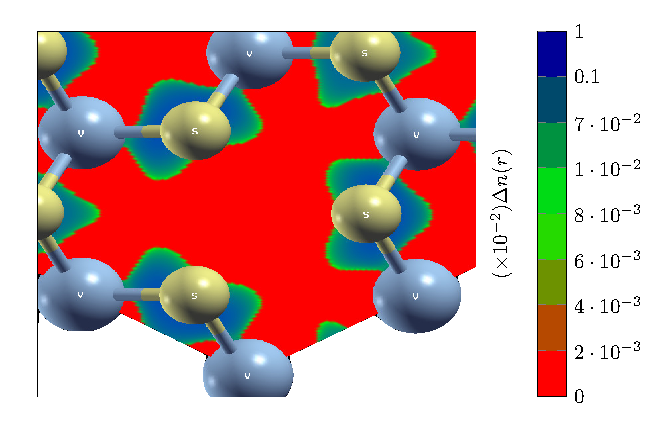
\epsfig{file=figRes/VS2/def/dens/densPos/densidadpos, scale=0.45}
			\label{Sim:fig:cargavacVS2}
		}
		\caption[densidad de carga en el VSe\textsubscript{2} yVS\textsubscript{2}]{densidad de carga en la regi\'on de la vacancia en el VSe\textsubscript{2} y VS\textsubscript{2} visualizada con XcrySDen }
		\label{Sim:fig:cargavacV}	
	\end{figure}
}
\frame{
	\frametitle{Vacancia de Vanadio en VSe\textsubscript{2} y VS\textsubscript{2}}
	\framesubtitle{Diagrama de bandas y densidad de estados del VSe\textsubscript{2}}
	
	\begin{figure}[!hbt]
		\centering
		\includegraphics[width=10cm, height=5cm]{figRes/VSe2/def/bandas/nosoc/bandasDOSnoSoc.pdf}
		\caption[diagrama de bandas y densidad de estados del VSe\textsubscript{2} con vacancia de Vanadio.]{Diagrama de bandas y la densidad de estados para el VSe\textsubscript{2}.} 
		\label{Sim:fig:VSe2noSOCcavband}
	\end{figure}
}
\frame{
	\frametitle{Vacancia de Vanadio en VSe\textsubscript{2} y VS\textsubscript{2}}
	\framesubtitle{Diagrama de bandas y densidad de estados del VS\textsubscript{2}}
	\begin{figure}[!hbt]
		\centering
		\includegraphics[scale=0.7]{figRes/VS2/def/bandas/nosoc/bandasDOSnoSoc.pdf}
		\caption[Diagrama de bandas  y densidad de estados en el VS\textsubscript{2} con vacancia de Vanadio]{Diagrama de bandas y Densidad de Estados del  VS\textsubscript{2}.}
		\label{Sim:fig:VacVS2bandas}
	\end{figure}
}
\frame{
	\frametitle{Vacancia de Vanadio en VSe\textsubscript{2} y VS\textsubscript{2}}
	\framesubtitle{Densidad de carga en VSe\textsubscript{2} y VS\textsubscript{2}}
	\begin{figure}[!hbt]
		\centering
		\subfigure[VSe\textsubscript{2}]{
			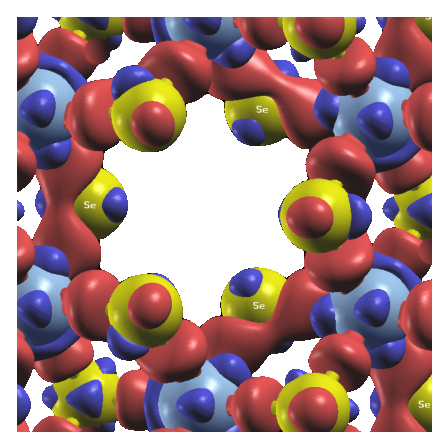
\epsfig{file=figRes/VSe2/def/densidad/vse2_carga_vac.eps, scale=0.6}
			\label{Sim:fig:cargaVacVSe2}
		}
		\subfigure[VS\textsubscript{2}]{
			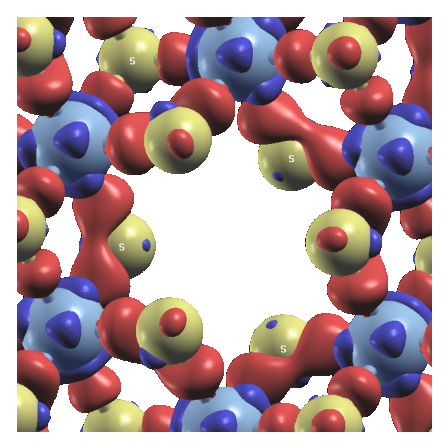
\epsfig{file=figRes/VS2/def/dens/vs2_carga_vac.eps, scale=0.6}
			\label{Sim:fig:cargaVacVS2}
			
		}
		\caption[Densidad de electrones en el VSe\textsubscript{2} y VS\textsubscript{2} con vacancia de Vanadio.]{Iso superficies de la densidad de carga con  un valor de $\pm 0.001 e/\AA^3$}
		\label{Sim:fig:cargaVac}
	\end{figure}
}

\frame{
	\frametitle{Vacancia de Vanadio en VSe\textsubscript{2} y VS\textsubscript{2}}
	\framesubtitle{Densidad de spin en VSe\textsubscript{2} y VS\textsubscript{2}}
	
	\begin{figure}[!hbt]
		\centering
		\subfigure[VSe\textsubscript{2}]{
			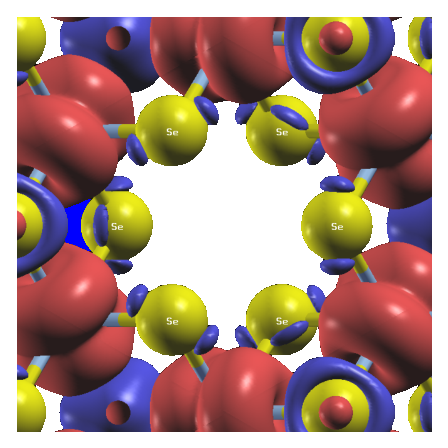
\epsfig{file=figRes/VSe2/def/densidad/vse2_magz.eps, scale=0.6}
			\label{Sim:fig:magnVacVSe2}
		}
		\subfigure[VS\textsubscript{2}]{
			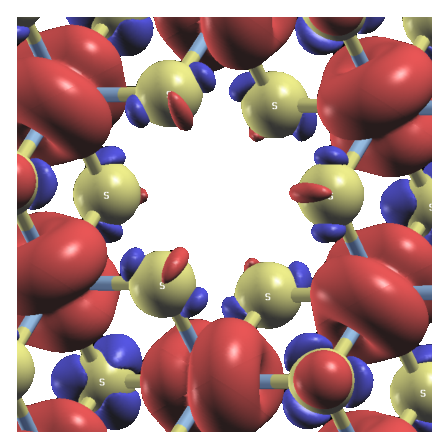
\epsfig{file=figRes/VS2/def/dens/vs2_magz.eps, scale=0.6}
			\label{Sim:fig:magnVacVS2}
			
		}
		\caption[Densidad de spin en el VSe\textsubscript{2} y VS\textsubscript{2} con vacancia de Vanadio.]{Iso superficies de la densidad de spines con  un valor de $\pm 0.0002 e/\AA^3$}
		\label{Sim:fig:magzVacV}
	\end{figure}
}
\subsubsection{Efectos de la deformaci\'on mec\'anica en la magnetizaci\'on}
\frame{
	\frametitle{Deformaci\'on isotr\'opica en VSe\textsubscript{2} y VS\textsubscript{2}}
	\framesubtitle{Magnetizaci\'on}
	\begin{figure}[!hbt]
		\centering
		\subfigure[VSe\textsubscript{2}]{
			\includegraphics[scale=0.55]{figRes/VSe2/str/isotropico/magn.pdf}
			\label{Sim:fig:strVSe2Iso}
		}
		\subfigure[VS\textsubscript{2}]{
			\includegraphics[scale=0.55]{figRes/VS2/str/isotropico/magn.pdf}
			\label{Sim:fig:strVS2Iso}
		}
		\caption[Magnetizaci\'on del VSe\textsubscript{2} y VS\textsubscript{2} en funci\'on de una deformaci\'on isotr\'opica. ]{Gr\'aficas de la magnetizaci\'on en funci\'on de la deformaci\'on isotr\'opica en VSe\textsubscript{2} y VS\textsubscript{2} mostrando el ajuste lineal de los datos.}
		\label{Sim:fig:MgnVx2Iso}
	\end{figure}
}
\frame{
	\frametitle{Deformaci\'on isotr\'opica en VSe\textsubscript{2} y VS\textsubscript{2}}
	\framesubtitle{An\'alisis de distancias}
	\begin{figure}[!hbt]
		\centering
		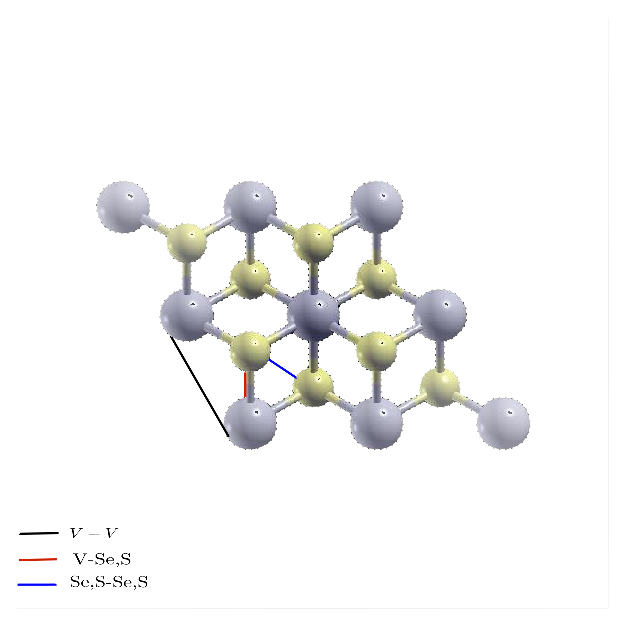
\epsfig{file=figRes/compIso,scale=0.5}
		\caption[ Distancias entre \'atomos   VSe\textsubscript{2} y VS\textsubscript{2} utilizados para el estudio de una deformaci\'on isotr\'opica]{Distancias entre \'atomos en el VSe\textsubscript{2} y  VS\textsubscript{2} en donde las esferas grises representran el vanadio y las amarillas El Azufre o Selenio.}
		\label{Sim:fig:disVX2Iso}
	\end{figure}
}
\frame{
	\frametitle{Deformaci\'on isotr\'opica en VSe\textsubscript{2} y VS\textsubscript{2}}
	\framesubtitle{Cambio en distancia entre \'atomo de Azufre o Selenio y Vanadio}
	\begin{figure}[!hbt]
		\centering
		\subfigure[VSe\textsubscript{2}]{
			\includegraphics[scale=0.55]{figRes/VSe2/str/isotropico/dVS.pdf}
			\label{Sim:fig:DVSVSe2Iso}
		}
		\subfigure[VS\textsubscript{2}]{
			\includegraphics[scale=0.55]{figRes/VS2/str/isotropico/dVS.pdf}
			\label{Sim:fig:DVSVS2Iso}
		}
		\caption[Cambio en la distancia entre \'atomos de Selenio o Azufre en  VSe\textsubscript{2} y VS\textsubscript{2} en funci\'on de una deformaci\'on isotr\'opica. ]{Cambio en la distancia entre dos \'atomos de Selenio en VSe\textsubscript{2} y Azufre en VS\textsubscript{2}.}
		\label{Sim:fig:DVSVx2Iso}
	\end{figure}
}
\frame{
	\frametitle{Deformaci\'on isotr\'opica en VSe\textsubscript{2} y VS\textsubscript{2}}
	\framesubtitle{magnetizaci\'on de cada \'atomo}
	\begin{figure}[!hbt]
		\centering
		\subfigure[VSe\textsubscript{2}]{
			\includegraphics[scale=0.4]{figRes/VSe2/str/isotropico/CompMag.pdf}
			\label{Sim:fig:cmagVse2I}	
		}
		\subfigure[VS\textsubscript{2}]{
			\includegraphics[scale=0.4]{figRes/VS2/str/isotropico/CompMag.pdf}
			\label{Sim:fig:cmagVs2I}	
		}
		\caption{magnetizaci\'on del \'atomo de vanadio y selenio o Azufre en el VSe2 (\ref{Sim:fig:cmagVse2I}) y VS\textsubscript{2} (\ref{Sim:fig:cmagVs2I}) bajo una deformaci\'on isotr\'opica.}
		\label{Sim:fig:cmagVX2I}
	\end{figure} 
}
\frame{
	\frametitle{Deformaci\'on anisotr\'opica en VSe\textsubscript{2} y VS\textsubscript{2}}
	\framesubtitle{Magnetizaci\'on}
	\begin{figure}[!hbt]
		\centering
		\subfigure[VSe\textsubscript{2}]{
			\includegraphics[scale=0.55]{figRes/VSe2/str/anisotropico/magn.pdf}
			\label{Sim:fig:strVSe2anis}
		}
		\subfigure[VS\textsubscript{2}]{
			\includegraphics[scale=0.55]{figRes/VS2/str/anisotropico/magn.pdf}
			\label{Sim:fig:strVS2Anis}
		}
		\caption[magnetizaci\'on del VSe\textsubscript{2} y VS\textsubscript{2} bajo una deformaci\'on anisotr\'opica.]{Gr\'aficas de la magnetizaci\'on en funci\'on de la deformaci\'on anisotr\'opica en VSe\textsubscript{2} y VS\textsubscript{2}.}
		\label{Sim:fig:MgnVx2Anis}
	\end{figure}
}
\frame{
	\frametitle{Deformaci\'on anisotr\'opica en VSe\textsubscript{2} y VS\textsubscript{2}}
	\framesubtitle{An\'alisis de distancias}
	\begin{figure}[!hbt]
		\centering
		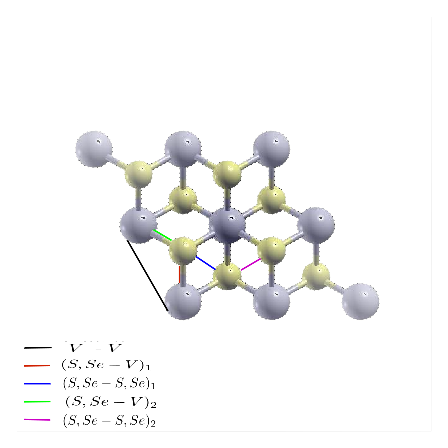
\epsfig{file=figRes/compAnis.eps,scale=0.6}
		\caption[Distancias entre \'atomos   VSe\textsubscript{2} y VS\textsubscript{2} utilizados para el estudio de una deformaci\'on aniisotr\'opica.]{Distancias entre \'atomos en el VSe\textsubscript{2} y  VS\textsubscript{2} en la deformaci\'on anisotr\'opica, las esferas grises representan el vanadio y las amarillas El Azufre o Selenio.}
		\label{Sim:fig:disVX2Anis}
	\end{figure}
}
\frame{
	\frametitle{Deformaci\'on anisotr\'opica en VSe\textsubscript{2} y VS\textsubscript{2}}
	\framesubtitle{Cambio en distancia entre \'atomo de Azufre o Selenio y Vanadio}
	\begin{figure}[!hbt]
		\centering
		\subfigure[VSe\textsubscript{2}]{
			\includegraphics[scale=0.55]{figRes/VSe2/str/anisotropico/CompdVS.pdf}
			\label{Sim:fig:compdSVVse2}	
		}
		\subfigure[VS\textsubscript{2}]{
			\includegraphics[scale=0.55]{figRes/VS2/str/anisotropico/CompdVS.pdf}
			\label{Sim:fig:compdSVVs2}	
		}
		\caption{variaci\'on de las distancias entre \'atomos de Selenio en el VSe\textsubscript{2} y de Azufre en VS\textsubscript{2}.}
		\label{Sim:fig:compdSVVX2}
	\end{figure}
}
\frame{
	\frametitle{Deformaci\'on anisotr\'opica en VSe\textsubscript{2} y VS\textsubscript{2}}
	\framesubtitle{magnetizaci\'on de cada \'atomo}
	\begin{figure}[!hbt]
		\centering
		\subfigure[VSe\textsubscript{2}]{
			\includegraphics[scale=0.4]{figRes/VSe2/str/anisotropico/CompMag.pdf}
			\label{Sim:fig:cmagVse2}	
		}
		\subfigure[VS\textsubscript{2}]{
			\includegraphics[scale=0.4]{figRes/VS2/str/anisotropico/CompMag.pdf}
			\label{Sim:fig:cmagVs2}	
		}
		\caption{magnetizaci\'on del \'atomo de vanadio y selenio o Azufre en el Vse2 (\ref{Sim:fig:cmagVse2}) y VS\textsubscript{2} (\ref{Sim:fig:cmagVs2}) bajo una deformaci\'on anisotr\'opica.}
		\label{Sim:fig:cmagVX2}
	\end{figure} 
}
%================================================================================================================
\frame{
	\frametitle{Deformaci\'on isotr\'opica en PtSe\textsubscript{2} y PtS\textsubscript{2}}
	\framesubtitle{Magnetizaci\'on}
	\begin{figure}[!hbt]
		\centering
		\subfigure[PtSe\textsubscript{2}]{
			\includegraphics[scale=0.5]{figRes/PtSe2/str/isotropico/magn.pdf}
			\label{Sim:fig:magnPtSe2}
		}
		\subfigure[PtS\textsubscript{2}]{
			\includegraphics[scale=0.5]{figRes/PtS2/str/isotropico/magn.pdf}
			\label{Sim:fig:magnPtS2}
			
		}
		\caption{Magnetizaci\'on en funci\'on de una deformaci\'on isotr\'opica en PtSe\textsubscript{2} y PtS\textsubscript{2} con una vacancia de Platino}
		\label{Sim:fig:magnPtX2}
	\end{figure}
}
\frame{
	\frametitle{Deformaci\'on isotr\'opica en PtSe\textsubscript{2} y PtS\textsubscript{2}}
	\framesubtitle{An\'alisis de distancias}
	\begin{figure}[htbp]
		\centering
		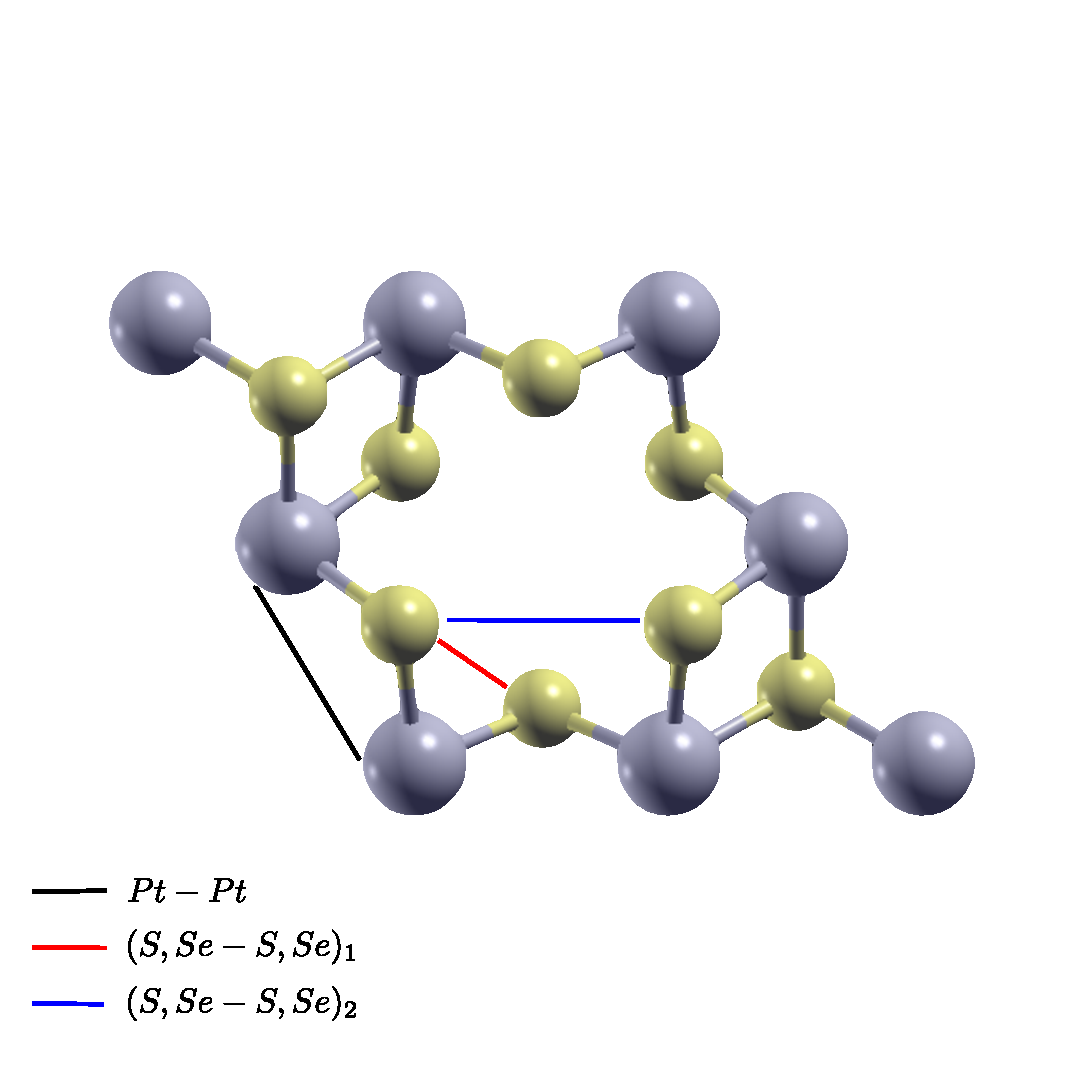
\epsfig{file=figRes/compIsoDef, scale=0.3}
		\caption{Distancias entre \'atomos que se utilizan para estudiar una desinformación isotrópica, las esferas grises representan los \'atomos de Platino y las amarillas a \'atomos de Selenio o  azufre. }
		\label{Sim:fig:defIsoPtX2}
	\end{figure}
}
\frame{
	\frametitle{Deformaci\'on isotr\'opica en PtSe\textsubscript{2} y PtS\textsubscript{2}}
	\framesubtitle{Cambio en distancia entre \'atomos de Azufre o Selenio}
	\begin{figure}[!hbt]
		\centering
		\subfigure[PtSe\textsubscript{2}]{
			\includegraphics[scale=0.45]{figRes/PtSe2/str/isotropico/CompdS.pdf}
			\label{Sim:fig:compdSePPtSe2}
		}
		\subfigure[PtS\textsubscript{2}]{
			\includegraphics[scale=0.45]{figRes/PtS2/str/isotropico/CompdS.pdf}
			\label{Sim:fig:compdSePPtS2}
		}
		\caption{Comparaci\'on del cambio entre \'atomos de Selenio en el PtSe\textsubscript{2} (\ref{Sim:fig:compdSePPtSe2}) y de Azufre en PtS\textsubscript{2} (\ref{Sim:fig:compdSePPtS2}.)
		}
		\label{Sim:fig:compdSePPtX2}
	\end{figure}
}
\frame{
	\frametitle{Deformaci\'on isotr\'opica en PtSe\textsubscript{2} y PtS\textsubscript{2}}
	\framesubtitle{magnetizaci\'on de cada \'atomo}
	\begin{figure}[!hbt]
		\centering
		\subfigure[PtSe\textsubscript{2}]{
			\includegraphics[scale=0.45]{figRes/PtSe2/str/isotropico/CompMagn.pdf}
			\label{Sim:fig:magnCptse2iso}
		}
		\subfigure[PtS\textsubscript{2}]{
			\includegraphics[scale=0.45]{figRes/PtS2/str/isotropico/CompMagn.pdf}
			\label{Sim:fig:magnCpts2iso}
		}
		\caption{magnetizaci\'on correspondiente a cada \'atomo de PtSe\textsubscript{2} yPtS\textsubscript{2} sujetos a una deformaci\'on isotr\'opica}
		\label{Sim:fig:magnCptx2iso}
	\end{figure}
}
\frame{
	\frametitle{Deformaci\'on anisotr\'opica en PtSe\textsubscript{2} y PtS\textsubscript{2}}
	\framesubtitle{Magnetizaci\'on}
	\begin{figure}[!hbt]
		\centering
		\subfigure[PtSe\textsubscript{2}]{
			\includegraphics[scale=0.5]{figRes/PtSe2/str/anisotropico/magn.pdf}
			\label{Sim:fig:magnPtSe2anis}
		}
		\subfigure[PtS\textsubscript{2}]{
			\includegraphics[scale=0.5]{figRes/PtS2/str/anisotropico/magn.pdf}
			\label{Sim:fig:magnPtS2anis}
			
		}
		\caption{Magnetizaci\'on en funci\'on de una deformaci\'on isotr\'opica en PtSe\textsubscript{2} y PtS\textsubscript{2} con una vacancia de Platino}
		\label{Sim:fig:magnPtX2anis}
		
	\end{figure}
}
\frame{
	\frametitle{Deformaci\'on anisotr\'opica en PtSe\textsubscript{2} y PtS\textsubscript{2}}
	\framesubtitle{An\'alisis de distancias}
	\begin{figure}[!hbt]
		\centering
		\includegraphics[scale=0.3]{figRes/compAnisDef.eps}
		\caption{Distancias entre \'atomos que se utilizan para estudiar una desinformación anisotr\'opica, las esferas grises representan los \'atomos de Platino y las amarillas a \'atomos de Selenio o  azufre. }
		\label{Sim:fig:defAnisPtX2}
	\end{figure}
}
\frame{
	\frametitle{Deformaci\'on anisotr\'opica en PtSe\textsubscript{2} y PtS\textsubscript{2}}
	\framesubtitle{Cambio en distancia entre \'atomos de Azufre o Selenio}
	\begin{figure}[!hbt]
		\centering
		\subfigure[PtSe\textsubscript{2}]{
			\includegraphics[scale=0.45]{figRes/PtSe2/str/anisotropico/CompdS.pdf}
			\label{Sim:fig:compdSePPtSe2A}
		}
		\subfigure[PtS\textsubscript{2}]{
			\includegraphics[scale=0.45]{figRes/PtS2/str/anisotropico/CompdS.pdf}
			\label{Sim:fig:compdSePPtS2A}
		}
		\caption{Comparaci\'on del cambio entre \'atomos de Selenio en el PtSe\textsubscript{2} (\ref{Sim:fig:compdSePPtSe2A}) y de Azufre en PtS\textsubscript{2} (\ref{Sim:fig:compdSePPtS2A} )en una deformaci\'on anisotr\'opica.
		}
		\label{Sim:fig:compdSePPtX2A}
	\end{figure}
}
\frame{
	\frametitle{Deformaci\'on anisotr\'opica en PtSe\textsubscript{2} y PtS\textsubscript{2}}
	\framesubtitle{magnetizaci\'on de cada \'atomo}
	\begin{figure}[!hbt]
		\centering
		\subfigure[PtSe\textsubscript{2}]{
			\includegraphics[scale=0.45]{figRes/PtSe2/str/anisotropico/CompMagn.pdf}
			\label{Sim:fig:magnCptse2aniso}
		}
		\subfigure[PtS\textsubscript{2}]{
			\includegraphics[scale=0.45]{figRes/PtS2/str/anisotropico/CompMagn.pdf}
			\label{Sim:fig:magnCpts2aniso}
		}
		\caption{magnetizaci\'on correspondiente a cada \'atomo de PtSe\textsubscript{2} yPtS\textsubscript{2} de una deformaci\'on anisotr\'opica}
		\label{Sim:fig:magnCptx2aniso}
	\end{figure} 
}

